\section{Exercício 7}

    Faça um programa que contenha a função Potencia. Esta função deve ser capaz
    de receber dois valores \emph{V} e \emph{EXP} e ter como saída $V{exp}$.
    Esta saída deve estar associada ao acumulador

\subsection{Descrição Alto Nível}

A desrição em alto nível foi utilizando a linguagem python é desta forma:

\begin{lstlisting}

def pot(n, exp):
    res = 1
    while exp > 0:
        res = mult_sum(res, n)        
        exp -=1
    return res


def mult_sum(a, b):
    res = 0
    while b > 0:
        res += a
        b-=1
    return res

\end{lstlisting}
Note que foi usada uma função auxiliar para fazer a multiplicação atraveś de
soma isso para que a descrição em alto nível seja mais parecida com a
implementação de baixo nível. 

\subsection{Descrição Baixo nível}
\begin{verbatim}
    
.CODE
INIT:
	lda exp
	jz  FIM,R
	jsr MULT_SUM,R
	sta res
	lda exp
	add #-1
    sta exp
	jmp INIT
		MULT_SUM:
            lda #0
            sta resAux
		lda n
		sta aux
		LOOP2:
			jz FIMLOOP2,R
			add #-1
			sta aux
			lda resAux
			add res
			sta resAux
			lda aux
			jmp LOOP2,R
		FIMLOOP2:
			lda resAux
			rts
	FIM:
		hlt
.ENDCODE

.DATA
	n:		db	#3
	exp:		db	#3
	res:	db	#1      ;respota

	aux:	db	#0      
	resAux:	db	#0
.ENDDATA

\end{verbatim}

\subsection{Tela Montador}

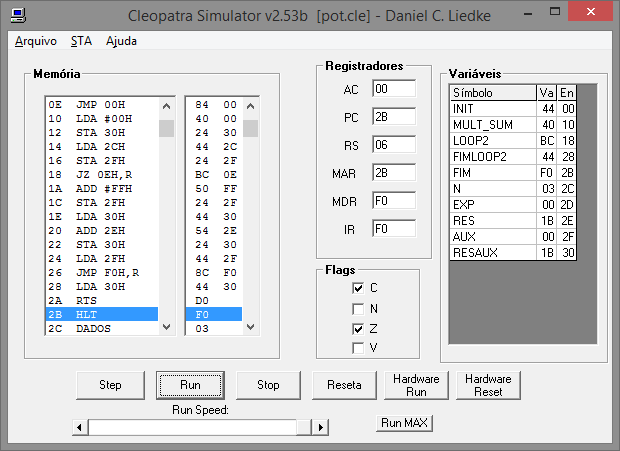
\includegraphics{images/pot.png}

\subsection{Contagem Operações e estimativa de de tempo de execução}

Considerando \emph{n} como \emph{x} e \emph{exp} como \emph{y} temos a seguinte função:
$$73y + 46xy + 39$$
O Tempo de excução seria 0.000672ms para x e y valendo 3, ao considerarmos que o Cleópatra opera a
1GHz.
